\addchapheadtotoc
\chapter{Background}
\section{The blended hardening technique}
\subsection{The double execution phase}
Double execution of a sequence of instructions consists in executing this sequence two times. To achieve this, the state of the system is saved, the sequence is executed a first time, then the system's state is restored to the initial state of the process before resuming the execution of the same sequence of instructions a second time. Currently, there is no ready-made instruction in processors to re-execute a sequence of instructions from a \cite{intel_corporation_intel_2011} program. So to achieve this, we use instruction counting to ensure that the two executions have exactly the same number of instructions. In practice, we let the program execute its instructions normally in a first phase (we have provided a mechanism to stop it if it takes too long), then we calculate the exact number of instructions contained in this first execution and we do so that the second execution has exactly the same number of instructions.

\section{Verification phase}
The verification is done by comparing the \acrshort {crc} code calculated on the modified memory range instead of conducting a word-by-word comparison. A word can contain 32 bits or 64 bits depending on the architecture of the processor. The method of the CRC code has the advantage of being faster and offers more possibility of re-using.

Although the initial objective is not yet fully achieved, we already have some results which we will detail in the next section.

\section{Architecture of generic hypervisor}
A hypervisor is a program that creates one or more virtual machines in each of which an OS can be run. The OS is no longer master of the system but is unaware of it; it is then designated by the term guest OS. We therefore modify the hypervisor to be able to protect the execution of the OS in a virtual machine. When the hypervisor is micro-kernel, we speak of micro-hypervisor. In this case, all the virtual machine management functionalities are outsourced to another program generally designated by the name of Virtual Machine Monitor (\acrshort{vmm}) which is like service application. The general diagram of a micro-kernel hypervisor is presented in figure \ref{fig: micro_hypervisor}.

The micro-hypervisor therefore directly controls the hardware and creates the virtual machines. Each guest OS is associated with a specific VMM which is capable of resolving the exceptions that this OS may raise. In practice, the micro-hypervisor redirects each sensitive operation that the guest OS initiates to its VMM which decides what to do. Hardening the micro-hypervisor, VMMs, other server applications and device drivers therefore makes it possible to support any OS.

\begin{figure}[h]
	\centering
	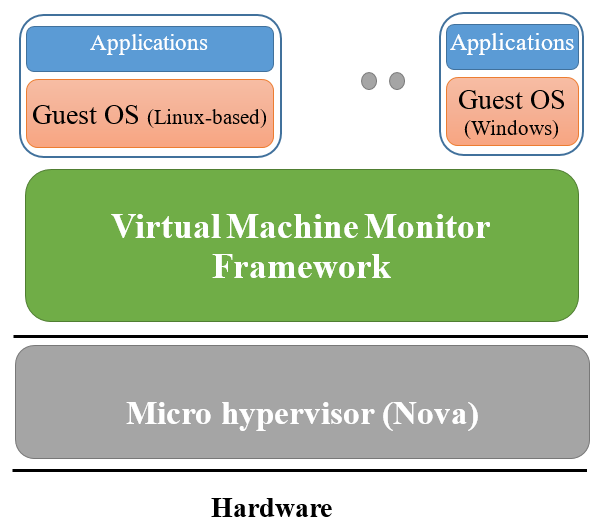
\includegraphics[width=0.5\textwidth]{image/micro_hypervisor}
	\caption{Schéma d'un micro-hyperviseur avec ses OS invités}
	\label{fig:micro_hypervisor}
\end{figure}